\documentclass[twoside, 11pt]{exam}

\usepackage[T1]{fontenc}
\usepackage[utf8]{inputenc}
\usepackage[dutch]{babel}

\usepackage[font={small,sf},labelfont={bf},labelsep=endash]{caption}
\usepackage{fouriernc}
\usepackage[detect-all, binary-units, separate-uncertainty=true,
            per-mode=symbol, retain-explicit-plus, range-phrase={ tot },
            list-final-separator={ en }, output-decimal-marker={,}]
            {siunitx}

\usepackage{setspace}
\setstretch{1.2}

\setlength{\parskip}{\smallskipamount}
\setlength{\parindent}{0pt}

\usepackage{geometry}
\geometry{a4paper, vmargin=3cm, inner=3cm, outer=2cm, head=14pt}

\usepackage{float}

\usepackage[fleqn]{amsmath}
\numberwithin{equation}{section}
\numberwithin{figure}{section}

\usepackage{graphicx}
\graphicspath{{Figures/}}
\usepackage{subfig}

\usepackage[svgnames]{xcolor}
\usepackage{tikz}
\usepackage{tikz-3dplot}
\usepackage{pgfplots}
\usetikzlibrary{plotmarks,circuits.ee.IEC,pgfplots.groupplots,external,calc}
\pgfplotsset{compat=1.3}

\usepackage{minted}
\usepackage{amsthm}
\usepackage{relsize}
\usepackage{xspace}
\usepackage{url}
\usepackage{sansmath}
\usepackage{titling}


\theoremstyle{plain}
\newtheorem*{note}{Note}


\newcommand{\figref}[1]{Figuur~\ref{#1}}

\newcommand{\hisparc}{\textsmaller{HiSPARC}\xspace}
\newcommand{\kascade}{\textsmaller{KASCADE}\xspace}
\newcommand{\sapphire}{\textsmaller{SAPPHiRE}\xspace}
\newcommand{\jsparc}{\textsmaller{jSparc}\xspace}
\newcommand{\hdf}{\textsmaller{HDF5}\xspace}
\newcommand{\aires}{\textsmaller{AIRES}\xspace}
\newcommand{\csv}{\textsmaller{CSV}\xspace}
\newcommand{\python}{\textsmaller{PYTHON}\xspace}
\newcommand{\corsika}{\textsmaller{CORSIKA}\xspace}
\newcommand{\labview}{\textsmaller{LabVIEW}\xspace}
\newcommand{\dspmon}{\textsmaller{DSPMon}\xspace}
\newcommand{\daq}{\textsmaller{DAQ}\xspace}
\newcommand{\adc}{\textsmaller{ADC}\xspace}
\newcommand{\adcs}{\textsmaller{ADC}s\xspace}
\newcommand{\Adcs}{A\textsmaller{DC}s\xspace}
\newcommand{\hi}{\textsc{h i}\xspace}
\newcommand{\hii}{\textsc{h ii}\xspace}
\newcommand{\mip}{\textsmaller{MIP}\xspace}
\newcommand{\hisparcii}{\textsmaller{HiSPARC II}\xspace}
\newcommand{\hisparciii}{\textsmaller{HiSPARC III}\xspace}
\newcommand{\pmt}{\textsmaller{PMT}\xspace}
\newcommand{\pmts}{\textsmaller{PMT}s\xspace}
\newcommand{\gps}{\textsmaller{GPS}\xspace}

\DeclareSIUnit{\electronvolt}{\ensuremath{\mathrm{e\!\!\:V}}}

\DeclareSIUnit{\unitsigma}{\ensuremath{\sigma}}
\DeclareSIUnit{\mip}{\textsmaller{MIP}}
\DeclareSIUnit{\adc}{\textsmaller{ADC}}

\DeclareSIUnit{\gauss}{G}
\DeclareSIUnit{\parsec}{pc}
\DeclareSIUnit{\year}{yr}


%% Document style definitions

% macros and commands
\newcommand{\shorttitle}[1]{\def\theshorttitle{#1}}
\newcommand{\docindex}[1]{\def\thedocindex{#1}}
\newcommand{\version}[1]{\def\theversion{#1}}
\newcommand{\setsectionstyle}[2]{
  \colorlet{seccolor}{#1}
  \def\thesectiontitle{#2}
}

\newcommand{\setdocumentstyle}[4]{
  \setsectionstyle{#1}{#2}
  \docindex{#3}
  \shorttitle{#4}
}

% document types
\newcommand{\docalgemeen}[2]{\setdocumentstyle{red}{Algemeen}{#1}{#2}}
\newcommand{\docinstallatie}[2]{\setdocumentstyle{Gold}{Detector installatie}{#1}{#2}}
\newcommand{\docdetector}[2]{\setdocumentstyle{blue}{Detector}{#1}{#2}}
\newcommand{\docweerstation}[2]{\setdocumentstyle{LightSlateGray}{Weerstation}{#1}{#2}}
\newcommand{\docbliksem}[2]{\setdocumentstyle{orange}{Bliksem}{#1}{#2}}
\newcommand{\docanalyse}[2]{\setdocumentstyle{DarkViolet}{Data analyse}{#1}{#2}}
\newcommand{\docwerkblad}[2]{\setdocumentstyle{ForestGreen}{Werkbladen}{#1}{#2}}
\newcommand{\docdocent}[2]{\setdocumentstyle{DarkKhaki}{Uitwerkingen}{#1}{#2}}
\newcommand{\docopdrachten}[2]{\setdocumentstyle{Silver}{Opdrachten}{#1}{#2}}
\newcommand{\docrecept}[2]{\setdocumentstyle{Navy}{Recept}{#1}{#2}}

\pgfmathsetlengthmacro\stylemarginsep{+1cm}
\pgfmathsetlengthmacro\stylethumbsep{+.75cm}

\newcommand{\rightthumb}{
\begin{tikzpicture}[remember picture, overlay]
  % vertical line
  \draw[seccolor]
    ($(current page.north east) + (-\stylemarginsep, -.5cm)$) --
    ($(current page.south east) + (-\stylemarginsep, .5cm)$);

  % thumb
  \fill[seccolor]
    ($(current page.north east) +
      (-\stylemarginsep, -2cm -\thedocindex * \stylethumbsep)$)
      rectangle +(.5cm, -.5cm);
\end{tikzpicture}
}

\newcommand{\leftthumb}{
\begin{tikzpicture}[remember picture, overlay]
  % vertical line
  \draw[seccolor]
    ($(current page.north west) + (\stylemarginsep, -.5cm)$) --
    ($(current page.south west) + (\stylemarginsep, .5cm)$);

  % thumb
  \fill[seccolor]
    ($(current page.north west) +
      (\stylemarginsep, -2cm -\thedocindex * \stylethumbsep)$)
      rectangle +(-.5cm, -.5cm);
\end{tikzpicture}
}

\renewcommand{\maketitle}{
  \suppressfloats

  \begin{titlepage}
  \thispagestyle{\defaultstyle}
  \let\endtitlepage\relax
  \begin{tikzpicture}[remember picture, overlay,
    titlebox/.append style={seccolor, fill, text=white, minimum height=1cm,
      font=\sffamily\huge, draw=none},
    authorbox/.append style={minimum height=.5cm, font=\sffamily}]

    \node[titlebox, anchor=north west, shift={(3cm, -1cm)}] at
      (current page.north west) {\thesectiontitle};

    \node[anchor=north west, shift={(2.83cm, -2cm)}] at
      (current page.north west) {
\includegraphics[scale=.8]{../HiSPARC_header}};

    \node[titlebox, anchor=north east, shift={(-\stylemarginsep, -1cm)}] at
      (current page.north east) {\thetitle};

    \node[authorbox, anchor=north east, shift={(-\stylemarginsep, -2cm)}] at
      (current page.north east) {\theauthor};
  \end{tikzpicture}
  \end{titlepage}
}


\newcommand{\defaultstyle}{headandfoot}

% style definitions
\pagestyle{\defaultstyle}
\chead{\oddeven{\rightthumb}{\leftthumb}}
\cfoot{\theshorttitle\ -- \thepage}
\lfoot{\oddeven{}{\textcolor{gray}{\smaller Versie \theversion}}}
\rfoot{\oddeven{\textcolor{gray}{\smaller Versie \theversion}}{}}

\renewcommand{\thequestion}{\textbf{Opdracht \arabic{question}:}}
\renewcommand{\solutiontitle}{\noindent\textbf{Antwoord:}\enspace}
\newcommand{\makelines}[1]{\ifprintanswers\else\fillwithlines{#1\linefillheight}\fi}

\ifdefined\showanswers
  \printanswers
\else
  \noprintanswers
\fi


\usepackage{hepnames} 
\usepackage[version=3]{mhchem}
\usepackage{lipsum}
\usepackage{pgfplots}
\usepackage{amsmath}
\usepackage{tikz}
\usetikzlibrary{shapes}
\usetikzlibrary{positioning,arrows}
\usetikzlibrary{decorations.pathmorphing}
\usetikzlibrary{decorations.markings}


\DeclareRobustCommand{\PgDpp}{\HepParticle{\Delta}{}{++}\xspace}

\title{Opdrachten: LHC Werkblad} 
\author{C.G.N. van Veen}
\docwerkblad{9}{LHC} 
\version{1.0}

\begin{document}

\maketitle

\section{Inleiding} In het voorjaar van 2015 start de LHC opnieuw op. Ditmaal 
met een hogere energie dan ooit tevoren. Protonen met een energie van \SI{7.0}{\tera\electronvolt}
zullen op elkaar botsen en bij deze botsingen hoopt men extra dimensies aan te tonen en 
aanwijzingen te vinden wat donkere materie is. Daarnaast zullen er interacties tussen Higgs bosonen 
onderzocht gaan worden.

\section{Voorkennis}

Van het natuurkunde programma van het VWO hebben leerlingen kennis nodig van impuls, 
energiebehoud,atoommodel en de beschikking hebben over een Binas.
Daarnaast hebben leerlingen geleerd dat geladen deeltjes afbuigen in magneetvelden en dat 
geladen deeltjes versneld kunnen worden in elektrische velden.
De energie van bewegende deeltjes (relativistisch) is:\\
$E^2 = E_0^2 + p^2 \cdot c^2 \rightarrow  E^2 = m_0^2 \cdot c^4 + p^2 \cdot c^2 $

Als achtergrondinformatie moet de LHC guide gedownload worden van de 
website van CERN en kan de presentatie van I. van Vulpen gebruikt worden. 
LHC-guide: \url{http://cds.cern.ch/record/1165534/files/CERN-Brochure-2009-003-Eng.pdf}
Presentatie LHC: \url{www.nikhef.nl/~ivov/Talks/2009_10_14_FomVisiteNikhef.ppt}

\section{Opgaven atoombouw}
\begin{questions}
\question
Schat de grootte van een goudatoom. (We gaan uit van een kubusvormig blokje met 
zijden van 1 cm.)
\makelines{4} 

\begin{figure}[h]
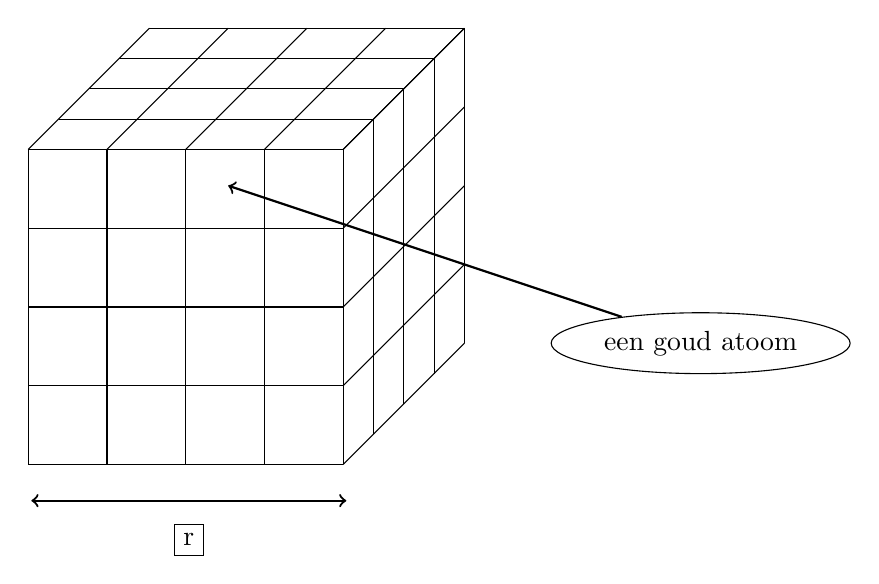
\begin{tikzpicture}
\foreach \x in{0,...,4}
{   \draw (0,\x ,4) -- (4,\x ,4);
    \draw (\x ,0,4) -- (\x ,4,4);
    \draw (4,\x ,4) -- (4,\x ,0);
    \draw (\x ,4,4) -- (\x ,4,0);
    \draw (4,0,\x ) -- (4,4,\x );
    \draw (0,4,\x ) -- (4,4,\x );
}
\coordinate (eindpijl) at (1,2);
\node [draw,ellipse] (start) at (7,0) {een goud atoom};
\draw [->, thick] (start) -- (eindpijl);
\draw [<->, thick] (-1.5,-2) -- (2.5,-2);
\node [draw] (begin) at (0.5,-2.5) {r};
\end{tikzpicture}
\end{figure}

\begin{solution}
De molaire massa van goud is \SI{197}{\gram\per\mol} en de dichtheid is 
\SI{19.3}{\gram\per\cubic\centi\meter}


$n = \frac{m}{M} = \frac{\rho \cdot V}{M} = 0,098 [mol]\\
N = n \cdot N_{A} = 5,9\cdot10^{22}$ \\
Er zijn $5,9\cdot 10^{22}$ atomen in de kubus van \SI{1.0}{\cubic\centi\meter} aanwezig.
$V = r^3 $ en $V^{'} = a^{3}$ \\Waar $V^{'} = \frac{V}{N}$ het volume dat een goudatoom in het rooster inneemt.\\
$a = \sqrt[3]{\frac{V}{N}} = 2,56\cdot 10^{-8} cm \approx 2,6 \cdot 10^{-10} m$
Als `a' de diameter is dan is de straal van het atoom is dus $\approx$ \SI{1e-10}{\meter}.
\end{solution}

\question
Welke energie is nodig om met elektronen de innerlijke structuur van \\
\begin{parts}

\part atomen te onderzoeken?\\
\makelines{4} 
\begin{solution}
Om de structuur van atomen te onderzoeken heb je een resolutie nodig van \SI{e-10}{\meter}.
Er geldt (voor atomen):\\
$p = \frac{h}{\lambda} = \frac{6,626\cdot 10^{-34}}{10^{-10}} = 6,626 \cdot 10^{-24} kgm/s$\\
$E_{kin} = \frac{p^2}{2m} = 150 eV$
Het gaat hier om niet relativistische elektronen omdat de benodigde energie minder is dan de rustenergie van elektronen.
\end{solution}

\part protonen en neutronen te onderzoeken?\\
(hint:Bedenk dat materie een golflengte heeft (de Broglie \footnote{zie routenet: \url{http://www.hisparc.nl/docent-student/lesmateriaal/routenet}}
) en dat de resolutie voor waarneming afhangt van de golflengte van het deeltje wat voor detectie moet zorgen.)

\makelines{4} 

\begin{solution}
Kerndeeltjes hebben afmetingen kleiner dan \SI{1e-15}{\meter}. 
Er geldt (voor kerndeeltjes):\\
$p = \frac{h}{\lambda} = \frac{6,626\cdot 10^{-34}}{10^{-15}} = 6,626 \cdot 10^{-29} kgm/s$\\
$E= \sqrt{p^{2}c^{2}+m_0^{2}c^{4}} \approx pc = 1,24 GeV$
Elektronen zijn met deze energie relativistisch. 
\end{solution}
\end{parts}

\question
Doordat we de afmetingen van neutronen en protonen weten, kunnen we schatten wat 
de massa is van het deeltje, dat voor de interactie tussen die twee zorgt.
Gebruik hierbij de onzekerheidsrelatie van Heisenberg en de tijd die een deeltje
nodig heeft om een afstand in de orde van grootte van een kerndeeltje af te leggen.
De afstand tussen twee nucleonen is in de orde van \SI{e-15}{m}.

\makelines{4} 
\begin{solution}
 
$r = c \cdot \Delta t \rightarrow \Delta t = \frac{r}{c} = \frac{10^{-15}}{3,0\cdot 10^{8}}= 3,34\cdot 10^{-24} s$

$\Delta E \cdot \Delta t \geq \hbar \rightarrow \Delta E = \frac {\hbar}{\Delta t} = 197 MeV$

$\hbar$ is $ \frac{h}{2\pi}$ 
De onzekerheidsrelatie voor een afstand van \SI{e-15}{m} geeft een afwijking in de energie van 
ongeveer \SI{200}{\mega\electronvolt}. Een deeltje wat zorgt voor een interactie tussen 
twee nucleonen zou dus een massa moeten hebben in de orde grootte van \SI{200}{\mega\electronvolt},
maar kan slechts \SI{e-24}{\second} bestaan. Yukawa voorspelde het $\pi$ -meson en Powell ontdekte het deeltje 
met een massa van \SI{140}{\mega\electronvolt}. Yukawa kreeg in 1949 de Nobelprijs.
\end{solution}

\begin{figure}
\caption{ Feynman voorstelling van sterke kernkracht door pionen.}
\tikzset{
particle/.style={thick,draw=blue, postaction={decorate},
    decoration={markings,mark=at position .5 with {\arrow[blue]{triangle 45}}}}
    }
\subfloat[proton, neutron interactie met uitwisseling van $\pi^0$.]
{

\begin{tikzpicture}

\coordinate(p1) at (2,2);
\coordinate(aux1) at (2,2);
\coordinate(p2) at (0,4);

\coordinate(n1) at (6,0);
\coordinate(n2) at (6,4);
\coordinate(aux2) at (4,2);

\draw[particle] (0, 0) node [left] {p} -- (p1) ;
\draw[particle] (p1) -- (p2) node [left] {p};
\draw[particle] (n1) node [right] {n} -- (aux2) ;
\draw[particle] (aux2) -- (n2) node [right] {n};
\draw[dotted, thick] (aux1) -- (aux2) node [midway, above] {$\pi^0$};
%\draw[gluon] (aux1) -- node[label=right:$\gamma$] {} (aux2);

\end{tikzpicture}
}
\subfloat[Interactie tussen p en n onder uitwisseling van een $\pi^{+}$]
{
\tikzset{
particle/.style={thick,draw=blue, postaction={decorate},
    decoration={markings,mark=at position .5 with {\arrow[blue]{triangle 45}}}}
    }
\begin{tikzpicture}

\coordinate(p1) at (2,2);
\coordinate(aux1) at (2,2);
\coordinate(p2) at (0,4);

\coordinate(n1) at (6,0);
\coordinate(n2) at (6,4);
\coordinate(aux2) at (4,2);

\draw[particle] (0,0) node [left] {p}  -- (p1) ;
\draw[particle] (p1) -- (p2) node [left] {n};
\draw[particle] (n1) node [right] {n} -- (aux2) ;
\draw[particle] (aux2) -- (n2) node [right] {p};
\draw[dotted, thick] (aux1) -- (aux2) node [midway, above] {$\pi^+$};
%\draw 
%\draw[gluon] (aux1) -- node[label=right:$\gamma$] {} (aux2);
\end{tikzpicture}
}

\label{fig:Pion_feynman}
\end{figure}

\section{ Versnellers}

In de LHC guide (die je kunt downloaden van de Cern site) vind je
informatie over de LHC en over de bundels protonen, die deze versneller
tot dichtbij de lichtsnelheid en vervolgens laat botsen in detectoren
zoals CMS en ATLAS. Om een betere voorstelling te kunnen maken gaan
we even rekenen aan de eigenschappen van de protonen bundels in de LHC.

\question
Vergelijk de dichtheid in een protonenbundel in de LHC met de dichtheid van zuurstof en goud 
(beide bij kamertemperatuur). Een bundel protonen is een cilinder met een lengte 
van \SI{15}{\centi\meter} en een straal van \SI{17e-6}{m}, met zo'n \SI{e11}{} protonen.
(We rekenen niet relativistisch vanuit de bundel zelf.)
 
\makelines{4} 
\begin{solution}

De dichtheid van goud kun je opzoeken in Binas. Dit tabellenboek geeft een waarde van 
$\rho$ is \SI{19.3}{\kilogram\per\cubic\meter}. Dit kun je omrekenen naar
een $\rho$ van \SI{19.3}{\gram\per\cubic\centi\meter}. 
Bij zuurstof gebruiken we dat er een mol zuurstof in \SI{22.4}{\liter} gaat.

$\rho_0 = \frac{n \cdot M}{V} = \frac {1 mol \cdot 16 g/mol}{22,4 L} = 7,14 \cdot 10^{-4} g/cm^{3} $

Voor de dichtheid in de bundel geldt:\\
$\rho_{bundel} = \frac{m}{V} = \frac{n_{p} \cdot m_{p}}{\pi \cdot r^2 \cdot l} \approx 1,23 \cdot 10^{-3} g/cm^{3}$

De dichtheid van de bundel is laag, maar heeft een iets grotere dichtheid dan een
gas.
\end{solution}

\section{LHC}

In de LHC guide kun je op pagina 30 veel specificaties opzoeken over de LHC.
\question
Zoek de omtrek van de LHC en de maximale magneetveldsterkte op van de 
supergeleidende magneten.
\makelines{2} 
\begin{solution}
blz. 30 $L = 26 659 [m] B = 8,33 [T]$
\end{solution}

\question 
Wat is de maximale energie, die een versneller met de lengte van de LHC en
het gegeven magneetveld, kan meegeven aan protonen? (hint: De middelpuntzoekende kracht wordt geleverd door
de Lorentzkracht.)

\makelines{6} 
\begin{solution}
In de ring bewegen geladen deeltjes met hoge snelheid, waarop het magneetveld
een lorentz kracht uitoefent. Deze Lorentz kracht levert de benodigde middelpuntzoekende
kracht op de bewegende protonen.

$F_L = F_{MPZ} \rightarrow q \cdot v \cdot B = \frac{m \cdot v^2}{R}$

De impuls van de bewegende protonen, wordt dan:

$ p = q \cdot R \cdot B $ \\
$   = 1,602 \cdot 10^{-19} \cdot \frac{27\cdot 10^3}{2\pi} \cdot 8,33 $ \\
$ \approx 5,756 \cdot 10^{-15} [kg\cdot m/s]$ \\
$ E \approx p.c \approx \frac{5,756 \cdot 10^{-15} \cdot 3,0 \cdot 10^8}{1,602 \cdot 10^{-19} [J/ev]} = 10,8 [TeV]$

\end{solution}

\question
Uit de vorige vraag vinden we dat de energie van de bundel hoger is dan \SI{7}{\tera\electronvolt},
die genoemd is in de LHC guide. De verklaring hiervoor is dat effectieve lengte (dat is de lengte waarin de protonen worden
afgebogen) korter is. Er zijn dus ook rechte stukken in de ring van de LHC.
Wat is dan effectieve lengte van de LHC uitgaande van de
\SI{7}{\tera\electronvolt}? De rustmassa van protonen is \SI{938}{\mega\electronvolt}.

\makelines{4} 
\begin{solution}
Volgens Einstein geldt:\\
$E^2 = E_0^2 + p^2 \cdot c^2 \rightarrow $
$p = \sqrt{\frac{E^2 -E_0^2}{c^2}} = \sqrt{\frac{7^2 -(938 \cdot 10^{-3})^2}{c^2}} \approx 7\frac{TeV}{c}$
De rustmassa van de protonen is dus te verwaarlozen bij deze hoge energiëen. 
Wat ook te verwachten was. 

Voor de impuls geldt geldt: \\
$p = \frac{E}{c} = \frac{7 \cdot 10^{12} \cdot 1,602 \cdot 10^{-19}}{3,0 \cdot 10^8} = 3,738 \cdot 10^{-15} [kg m/s]$

Het gedeelte van de LHC wat de bundel afbuigt is dan 
$ p = q \cdot R \cdot B $ \\
dus: \\
$R = \frac{m \cdot v}{q \cdot B} \rightarrow \frac{p}{q\cdot B} $
Voor de omtrek van de effectieve ring(2$\pi$R) vinden we: \\

$omtrek = 2 \pi \frac{p}{qB} = 2 \pi \frac{3,738 \cdot 10^{-15}}{1,602 \cdot 10^{-19} \cdot 8,36} \approx 17,5 [km]$

De effectieve lengte komt door het feit dat naast dat er magneten in de ring zijn
die de bundel protonen de bocht om buigen, er ook magneten zijn, die de protonenbundels focusseren.
De protonen worden ook versneld in gedeelten van de LHC ring.

Het gedeelte van de LHC, dat 'recht' is: \\
$ \frac{27 [km] - 17,5 [km]}{27 [km]} \approx 0,35$
\end{solution}

\question
Op bladzijde 34 van de LHC guide kun je lezen over de `proton beam' en dat elke beam bestaat
uit 2835 `bunches' van \SI{e11}{} protonen. Deze bunches botsen met elkaar op de plekken waar 
hun banen elkaar kruisen.
\begin{parts}
\part Hoeveel botsingen van deze `bunches' zijn er per seconde?

\makelines{4} 
\begin{solution}
De bunches reizen met de lichtsnelheid dus komen elke:
$t = \frac{L_{LHC}}{2835} / c = \frac{27\cdot 10^3}{2835} / 3,0 \cdot 10^8 = 3,2 .10^{-8} [s]$
Het aantal botsingen is dan: \\
$f = \frac{1}{3,0 \cdot 10^8} = 32 [MHz]$
Dit is minder dan de LHC guide aangeeft, maar dit komt door het 'pacman' effect.
Bundels die overblijven voegen samen met andere bundels.
\end{solution}

\part Hoeveel botsingen zijn er in een run (een run duurt ongeveer 10 uur)?

\makelines{2} 
\begin{solution}
In een uur hebben we dan:
$ 32\cdot10^6 \cdot 10 \cdot 3600 \approx 1,2\cdot 10^{12}$ botsingen.
\end{solution}
\end{parts}

\question 
Als een Formule 1 coureur met \SI{320}{\kilo\meter\per\hour} door de ring van de 
LHC zou rijden. Hoe lang moet hij rijden zodat hij dezelfde afstand heeft gereden als
proton in de LHC in 1 s aflegt?

\makelines{3} 
\begin{solution}
Het duurt dan: \\
$t = \frac{s}{v} = \frac{c\cdot t}{v} = \frac{ 300000 [km/s] \cdot 1 [s]}{320 [km/h]} = 937,5 [h] = 39 dagen.$
\end{solution}

\question
De LHC werkt met supergeleidende magneten, als deze aangezet worden kan de stroomsterkte
in de magneten toenemen met \SI{10}{\ampere\per\second}. Hoe lang duurt het dan om
de maximale stroomsterkte van \SI{11,7e3}{\ampere} te bereiken?

\makelines{4} 
\begin{solution}
De tijd, die dat kost is: \\
$t = \frac{11700 [A]}{10 [A/s]} = 1170 s \approx 19,5 [min.]$
\end{solution}

\question
Een buis in een deel van de LHC is ongeveer \SI{15}{\meter} lang en gemaakt van staal.
Hoeveel \SI{}{\centi\meter} is de buis kleiner geworden als hij van kamertemperatuur \SI{20}{\celsius}
naar \SI{1,9}{\kelvin} afgekoeld wordt?

\makelines{4} 
\begin{solution}
De lineaire expansiecoefficiënt $\lambda$ van staal is \SI{12e-6}{\per\kelvin}:\\
$\Delta L = L_0 \cdot \lambda \cdot \Delta T$
Invullen geeft:\\
$\Delta L = 15 \cdot 12\cdot 10^{-6} \cdot (293-1,9) = 0,05 [m]$
\end{solution}

\question
Hoeveel energie zit er in het totale aantal bundels protonen, die in één ring ronddraaien?
De energie van de protonen is \SI{7}{\tera\electronvolt} en er zitten \SI{e11}{} protonen in 
een bundel. 

\makelines{4} 
\begin{solution}
De totale energie in de bundel is:
$ E_{totaal} = 2835 \cdot 10^{11} \cdot 7 \cdot 10^{12} \cdot 1,602 \cdot 10^{-19} \approx 320 [MJ]$

Als je dit zou vergelijken met een boot die \SI{11}{\kilo\meter\per\hour} vaart. Dan 
heeft die boot een massa van :
$m = \sqrt{\frac{2 \cdot E}{v^2}} = \sqrt{\frac{2 \cdot 320 \cdot 10^6}{(11/3,6)^2}} = 7,0 \cdot 10^7 [kg] $

Er zit dus ontzettend veel energie in één beam protonen.
\end{solution}



























\end{questions} 
\end{document}
